% LaTeX file for Chapter 03


\chapter{Results}

\section{Exploratory Data Analysis}

\subsection{Mouse kidney cells} \label{mouse_dataset}
The first data set stems from a paper that investigates potential cellular targets of kidney disease in mice \citep{mouse_cells}. The authors isolated and sequenced a total of 57'979 cells from whole kidney cell suspensions (one kidney per mouse) derived from seven healthy male mice using droplet-based single-cell RNA sequencing. The samples were labelled as: normal1, normal2, normal3, normal4, Ksp-cre-GFP, Scl-cre-GFP and Pod-cre-GFP. For our work, we decided to use the raw data from the four samples that were labelled as normal to ensure the biological reproducibility between the samples.

We used the \emph{alevin-fry} pipeline to quantify the raw single-cell RNA sequencing data for further use in the R programming environment. Quality control is a crucial stage in data pre-processing as low-quality libraries can contribute to misleading results in downstream analyses \citep{OSCA}. Therefore, we filtered lowly abundant genes and low-quality cells to mitigate said problems to improve interpretability of the results. 

To identify low-quality cells, cell-specific QC metrics were calculated with the \emph{perCellQCMetrics} function from the \emph{scater} R package \citep{scater}. These metrics include the total number of expressed genes, the overall count across all genes, and the fraction of counts assigned to control genes such as mitochondrial genes. By setting a specific threshold on per-cell QC metrics, high-quality cells can be retained. In our setting, outliers are defined as cells with library sizes more than two median absolute deviations away from the median library size. Figure \ref{fig:QC} summarizes the process from unprocessed to processed single-cell experiment. 

\begin{figure}[!htb]
\begin{center}
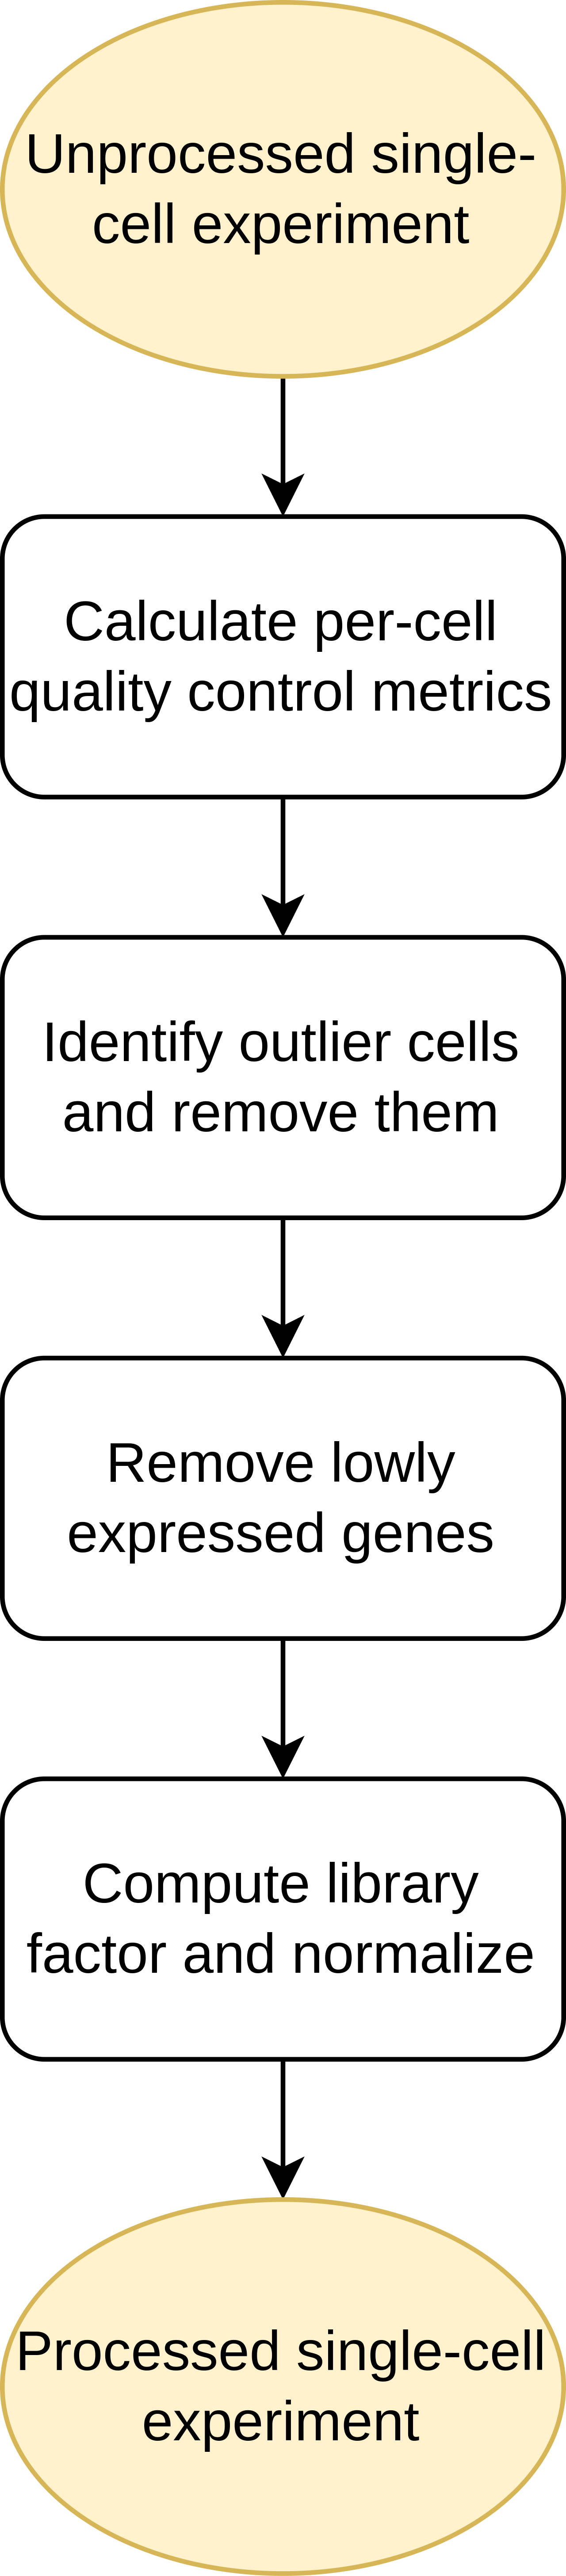
\includegraphics[width=1.5in,height=6in]{figure/qc.png}
\end{center}
\caption{Quality control process from unprocessed, raw to processed, filtered single-cell experiment}
\label{fig:QC}
\end{figure}
\FloatBarrier

After filtering, the data set consists of 23'543 cells and 18'537 genes. Next, we used the \emph{singleR} function from the \emph{singleR} R package \citep{singleR} for cell-type annotation. Cell-type annotation is important to determine what biological state is represented by cell clusters which helps the interpretability of the results and their implications \citep{OSCA}. \emph{singleR} is a method that assigns labels based on the reference samples with the highest Spearman rank correlation while only using marker genes between pairs of labels to focus on the relevant differences between cell types \citep{singleR}. Figure \ref{fig:UMAP_mouse_sample_id} shows the Uniform Manifold Approximation and Projection (UMAP) of the cells coloured by their respective sample id. From Figure \ref{fig:UMAP_mouse_sample_id} one can observe that the projection of the cells is very similar across the samples. Further, Figure \ref{fig:UMAP_mouse_cell_type} also illustrates that cells from the same cell-type cluster together, as one would expect.

Figure \ref{fig:mouse_cell_type} shows that the annotated cells were largely classified as either: Adipocytes, Epithelial cells and Hepatocytes. Additionally, one can observe that those three cell types are approximately evenly distributed across the four samples. For further analyses we focus on those cell types to investigate the performance of existing methods for the detection of differentially expressed genes and design our own simulation study.

\begin{figure}[!htb]
\begin{center}
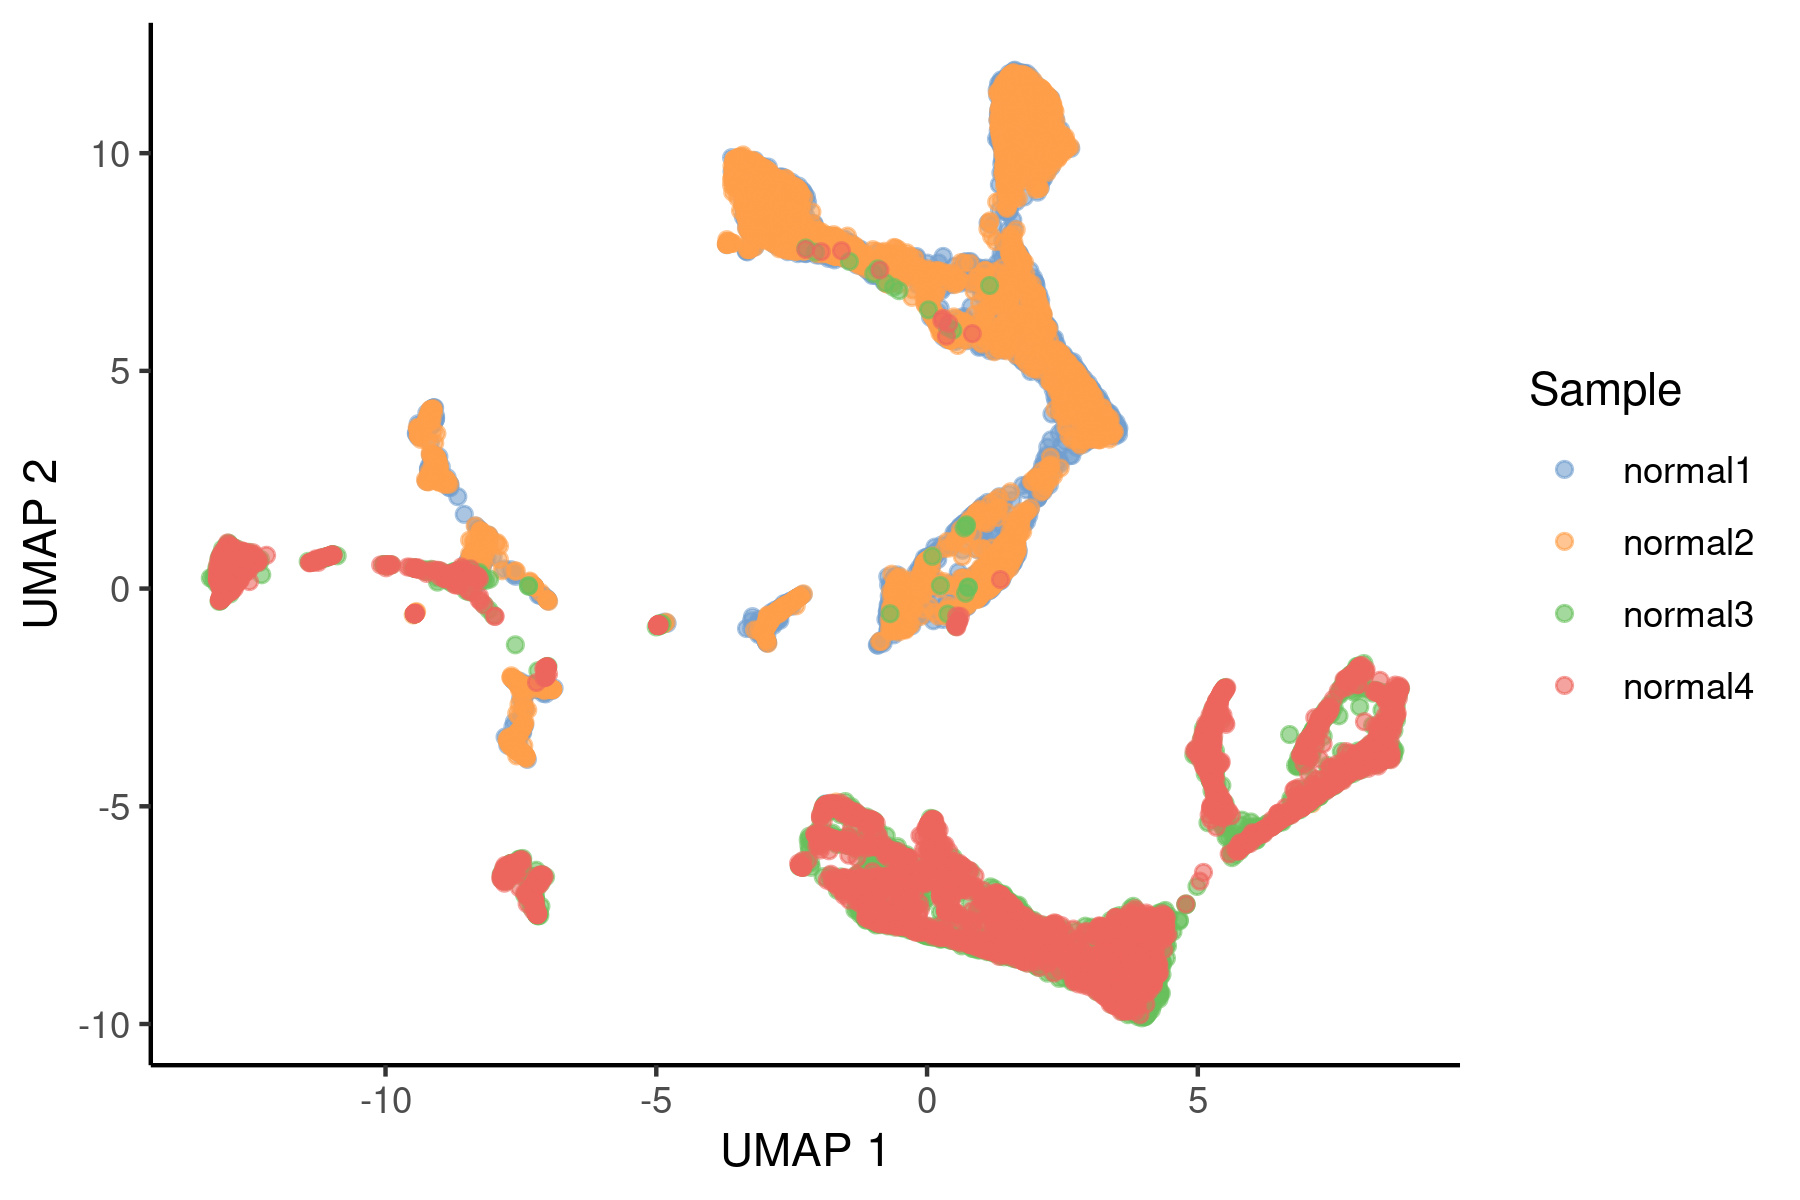
\includegraphics[width=6in,height=4in]{figure/kidney_mouse/UMAP_mouse_sample_id.png}
\end{center}
\caption{UMAP representation of the mouse kidney cells coloured by sample id}
\label{fig:UMAP_mouse_sample_id}
\end{figure}
\FloatBarrier

\begin{figure}[!htb]
\begin{center}
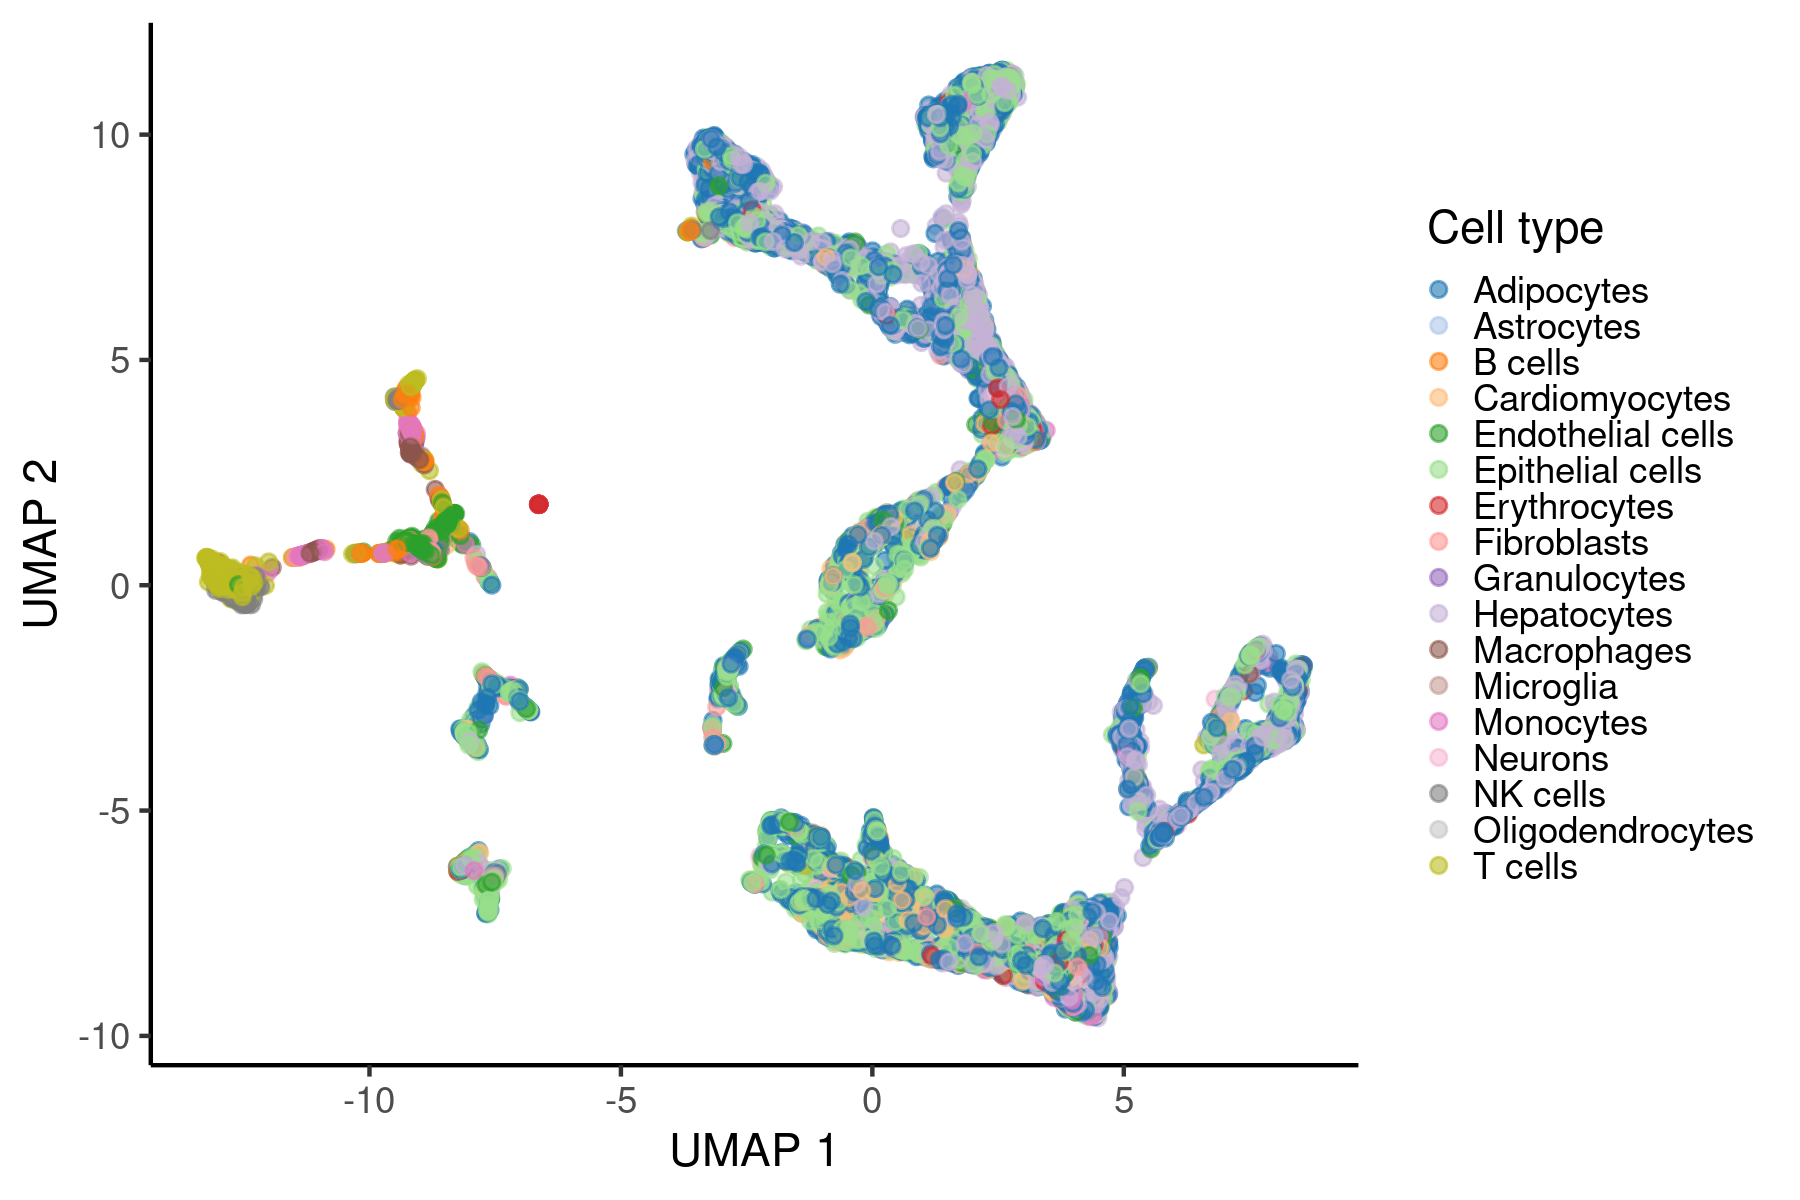
\includegraphics[width=6in,height=4in]{figure/kidney_mouse/UMAP_mouse_cell_type.png}
\end{center}
\caption{UMAP representation of the mouse kidney cells coloured by cell type}
\label{fig:UMAP_mouse_cell_type}
\end{figure}
\FloatBarrier

\begin{figure}[!htb]
\begin{center}
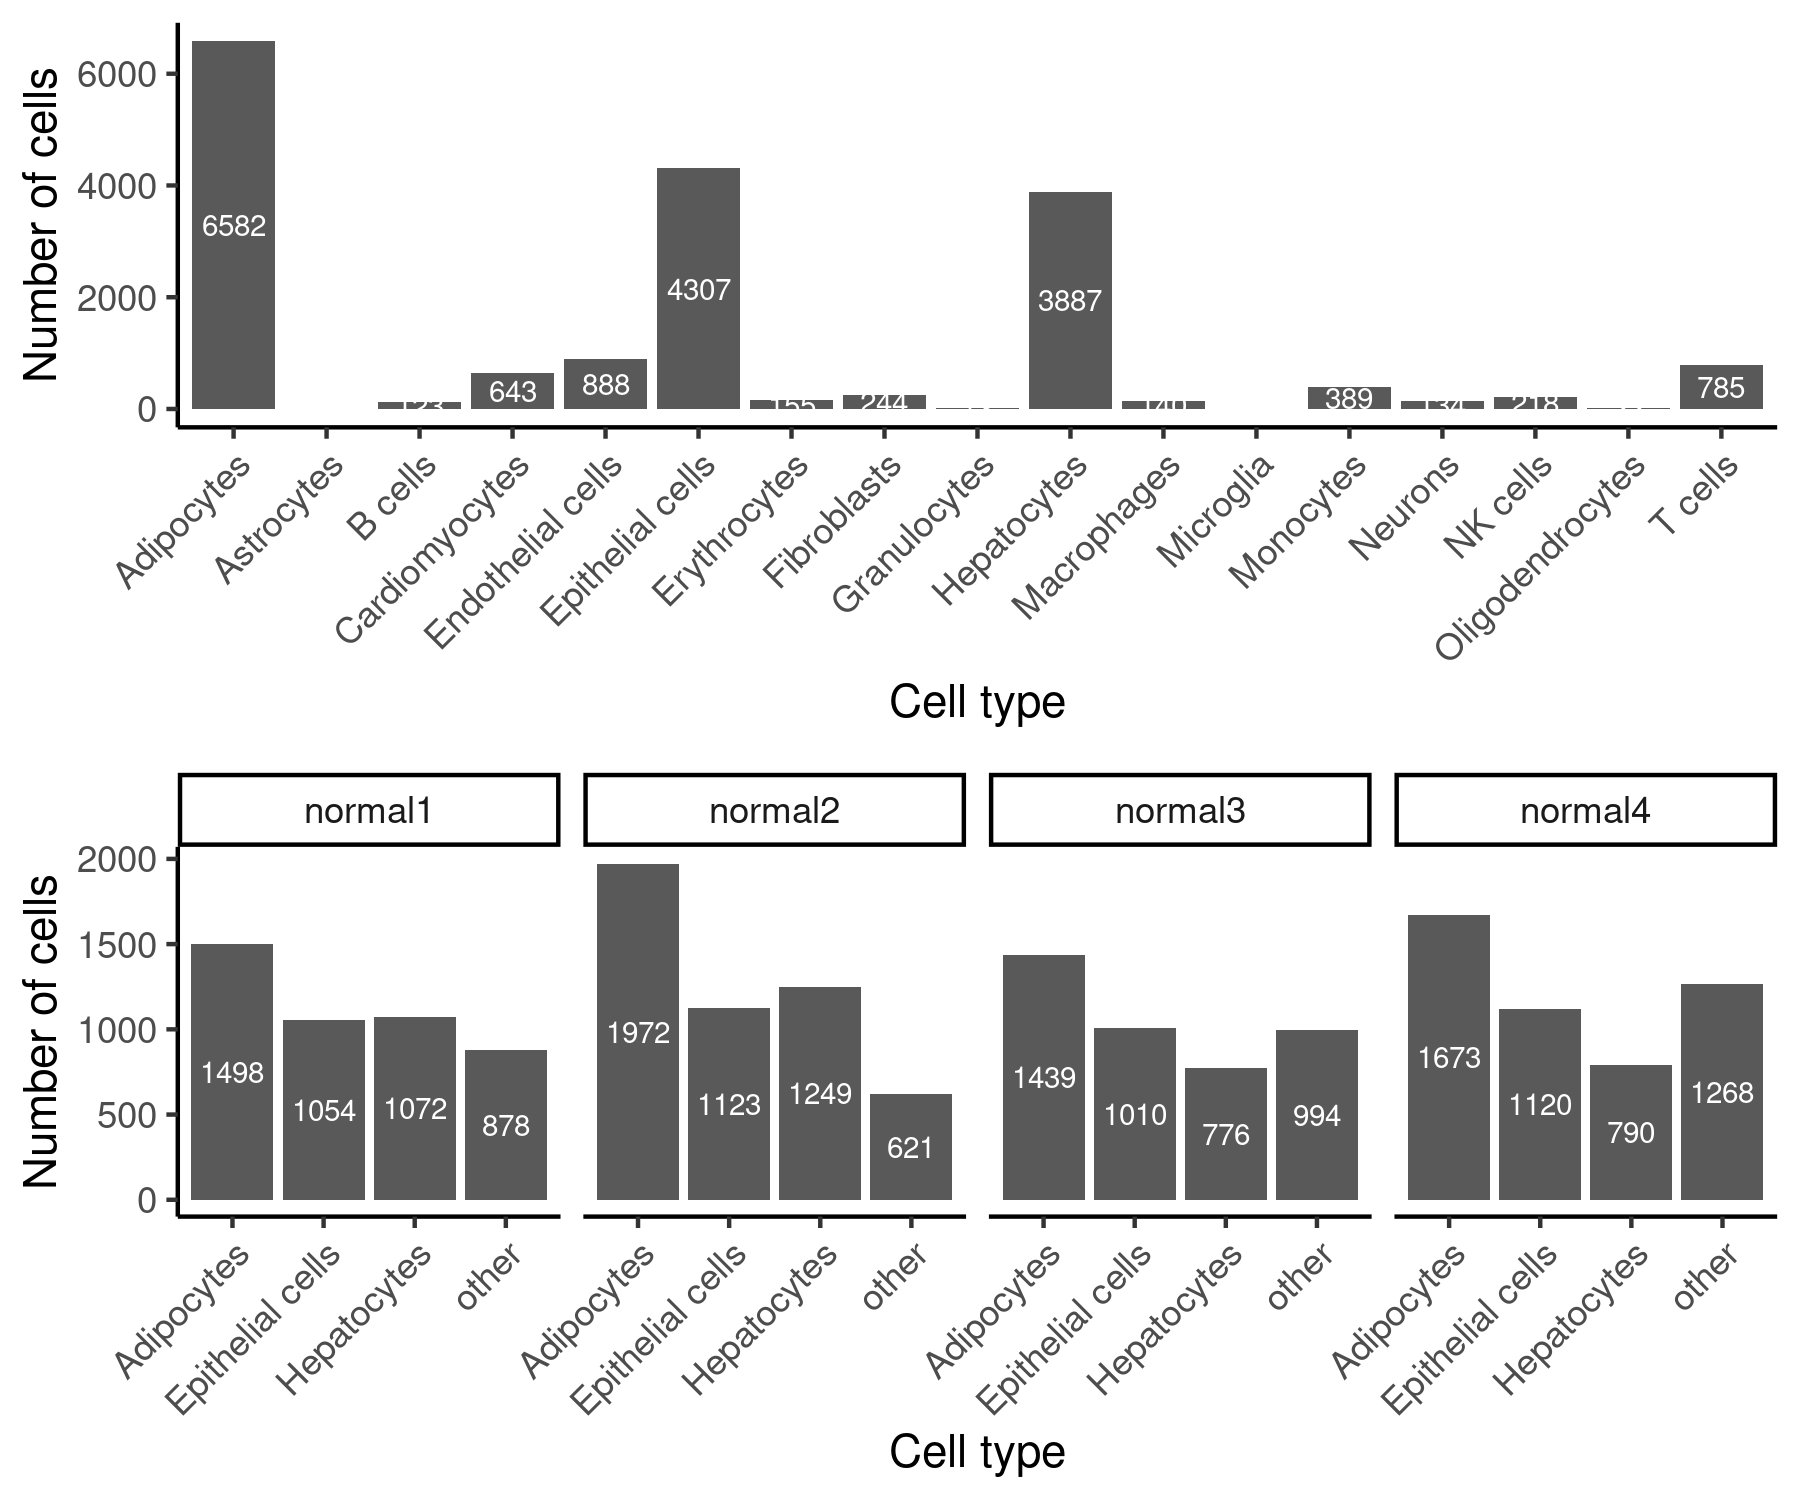
\includegraphics[width=6in,height=5in]{figure/kidney_mouse/cell_type_distribution.png}
\end{center}
\caption{Frequency distribution of the cell types after quality control} 
\label{fig:mouse_cell_type}
\end{figure}
\FloatBarrier

\subsection{RNA Velocity analysis}

\section{Simulation study}

\subsection{Simulation strategy}
Initially, the simulation strategy was to invert the spliced and unspliced counts for 10\% of genes for all cells that belong to an arbitrary group A. The set of genes whose counts were to be inverted was randomly drawn by a sampling algorithm without replacement (hypergeometric distribution). There are many different ways to introduce a differential effect, however nailing down on inverting the spliced and unspliced counts seemed like a neat way to do this without actually modifying the values. Additionally, differential gene expression was introduced in 10\% of genes in all cells that belong to said arbitrary group A. This was achieved by multiplying the counts (ten-fold gene expression) for 10\% randomly drawn genes in group A. Again, the set of genes was randomly drawn by the same sampling algorithm as before. In this manner two datasets were created, one with and one without differential gene expression. The genes and cells that were subject to change were stored as ground truth for further evaluation in the downstream analyses. Figure \ref{fig:simulation_process} illustrates the simulation process from the original mouse kidney data set to two simulated data sets.

\begin{figure}[!htb]
\begin{center}
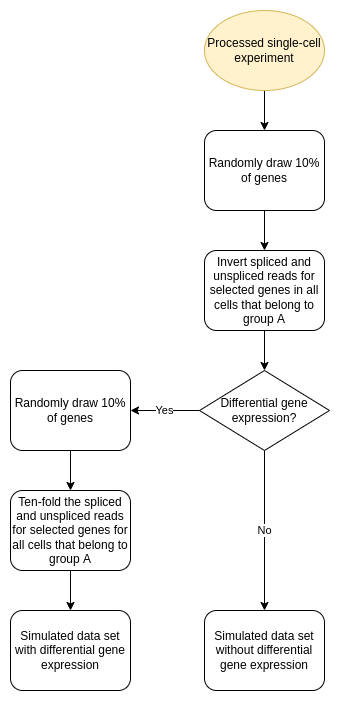
\includegraphics[width=3in,height=6in]{figure/kidney_mouse/first_simulation_process.png}
\end{center}
\caption{Simulation process from original mouse data set to simulated data sets}
\label{fig:simulation_process}
\end{figure}
\FloatBarrier

The goal of this thesis was to determine how well the aforementioned methods perform on detecting differentially regulated genes on read-level simulated data sets. To achieve this two groups of methods were postulated as \emph{eisaR} and \emph{BRIE2} cannot take into account ambiguous counts that are neither spliced or unspliced. For this reason the classification performance of \emph{eisaR} and \emph{BRIE2} are compared with each other with the help of ROC and TPR v. FDR curves. As alevin-fry allows the estimation of ambiguous counts as well as spliced and unspliced it was possible to assign the ambiguous counts to both spliced and unspliced counts (50-50 split) so that \emph{eisaR} and \emph{BRIE2} can be applied. In a similar manner, \emph{DEXSeq} and our own method were used to detect differentially regulated genes. However, in this case the ambiguous counts were used as an additional information rather than discarding it. As a next step, \emph{minnow} was used to introduce mapping uncertainty in the simulated data sets. After quantification of the new data sets the same performance protocol was used to assess the performance of all four methods.

\subsection{Preliminary results of the simple simulation}

\subsection{Read-level simulation with \emph{minnow}}

\section{Null data analysis on the mouse kidney data}

\section{Computational benchmark}

\section{Data availability}

\noindent\textbf{Kidney mouse cells} \\
The raw data can be downloaded from NCBI GEO (accession number GSE107585). \\ 
\url{https://www.ncbi.nlm.nih.gov/geo/query/acc.cgi?acc=GSE107585} \\

\section{Code availability}
All code for data preprocessing and analysis associated with the thesis is available at \url{https://github.com/joelmeili/DifferentialRegulation}. Any updates will also be published on GitHub.
